% Options for packages loaded elsewhere
\PassOptionsToPackage{unicode}{hyperref}
\PassOptionsToPackage{hyphens}{url}
%
\documentclass[
]{article}
\usepackage{lmodern}
\usepackage{amssymb,amsmath}
\usepackage{ifxetex,ifluatex}
\ifnum 0\ifxetex 1\fi\ifluatex 1\fi=0 % if pdftex
  \usepackage[T1]{fontenc}
  \usepackage[utf8]{inputenc}
  \usepackage{textcomp} % provide euro and other symbols
\else % if luatex or xetex
  \usepackage{unicode-math}
  \defaultfontfeatures{Scale=MatchLowercase}
  \defaultfontfeatures[\rmfamily]{Ligatures=TeX,Scale=1}
\fi
% Use upquote if available, for straight quotes in verbatim environments
\IfFileExists{upquote.sty}{\usepackage{upquote}}{}
\IfFileExists{microtype.sty}{% use microtype if available
  \usepackage[]{microtype}
  \UseMicrotypeSet[protrusion]{basicmath} % disable protrusion for tt fonts
}{}
\makeatletter
\@ifundefined{KOMAClassName}{% if non-KOMA class
  \IfFileExists{parskip.sty}{%
    \usepackage{parskip}
  }{% else
    \setlength{\parindent}{0pt}
    \setlength{\parskip}{6pt plus 2pt minus 1pt}}
}{% if KOMA class
  \KOMAoptions{parskip=half}}
\makeatother
\usepackage{xcolor}
\IfFileExists{xurl.sty}{\usepackage{xurl}}{} % add URL line breaks if available
\IfFileExists{bookmark.sty}{\usepackage{bookmark}}{\usepackage{hyperref}}
\hypersetup{
  pdftitle={Puromycin Practice},
  pdfauthor={Haley Reed},
  hidelinks,
  pdfcreator={LaTeX via pandoc}}
\urlstyle{same} % disable monospaced font for URLs
\usepackage[margin=1in]{geometry}
\usepackage{longtable,booktabs}
% Correct order of tables after \paragraph or \subparagraph
\usepackage{etoolbox}
\makeatletter
\patchcmd\longtable{\par}{\if@noskipsec\mbox{}\fi\par}{}{}
\makeatother
% Allow footnotes in longtable head/foot
\IfFileExists{footnotehyper.sty}{\usepackage{footnotehyper}}{\usepackage{footnote}}
\makesavenoteenv{longtable}
\usepackage{graphicx,grffile}
\makeatletter
\def\maxwidth{\ifdim\Gin@nat@width>\linewidth\linewidth\else\Gin@nat@width\fi}
\def\maxheight{\ifdim\Gin@nat@height>\textheight\textheight\else\Gin@nat@height\fi}
\makeatother
% Scale images if necessary, so that they will not overflow the page
% margins by default, and it is still possible to overwrite the defaults
% using explicit options in \includegraphics[width, height, ...]{}
\setkeys{Gin}{width=\maxwidth,height=\maxheight,keepaspectratio}
% Set default figure placement to htbp
\makeatletter
\def\fps@figure{htbp}
\makeatother
\setlength{\emergencystretch}{3em} % prevent overfull lines
\providecommand{\tightlist}{%
  \setlength{\itemsep}{0pt}\setlength{\parskip}{0pt}}
\setcounter{secnumdepth}{-\maxdimen} % remove section numbering

\title{Puromycin Practice}
\author{Haley Reed}
\date{5/27/2020}

\begin{document}
\maketitle

\textbf{Introduction}

It is relevant to explore the effects and reaction times of Puromycin
for its' application in biology. This report will use the data collected
by Margret Treloar in 1974 in extermination with rat livers to explore
these reaction times. Using this data obtained from R, this report will
explore how substrate concentration (measured in parts per million) and
the presence (or lack thereof) of the antibiotic Puromycin can act as
explanatory variables and model the reaction rate of enzymes. The rate,
our dependent variable, is measured by the number of counts per minute
of radioactive product.

\textbf{Analysis}

To begin our exploration of the data, we start with a scatterplot of the
rate represented by the explanatory variable concentration and
differentiate treated with black pointed and untreated with red.
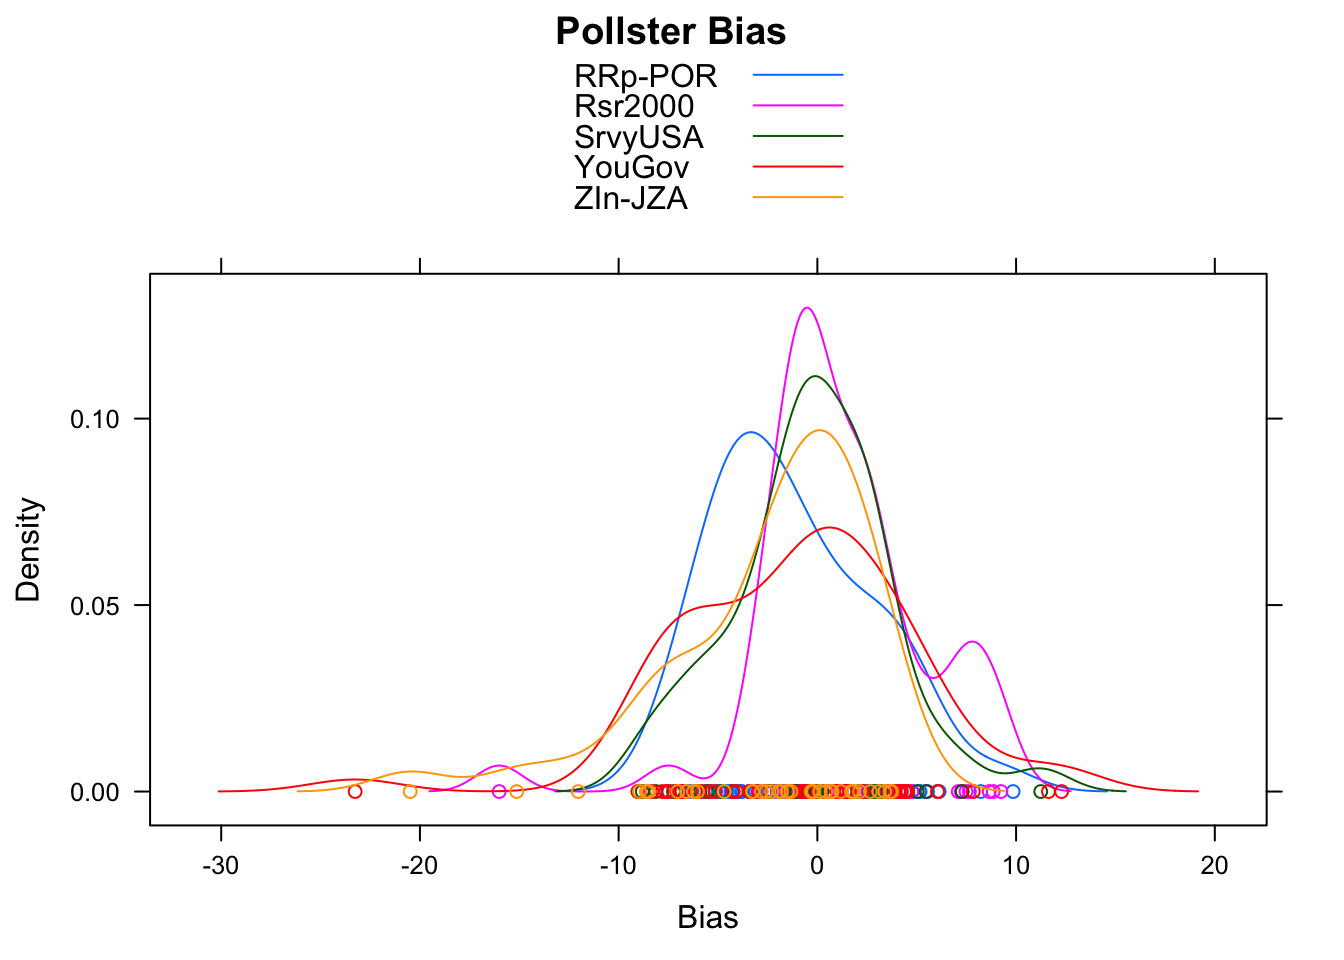
\includegraphics{Puromycin-R-Markdown-Practice_files/figure-latex/unnamed-chunk-1-1.pdf}

The data appears to be skewed to the right. The untreated data points
appear to have reactions that may have statistically significantly
slower reaction rates. The patterns present in this scatterplot
demonstrate that it would be helpful to build a model based on both
concentration and state (treated or untreated) to model reaction rates.
There appears to be a moderately strong positive relationship between
the two variables of concentration, however the relationship appears to
not be particularly linear. To address concerns of linearity, we will
apply a logarithmic transformation to the numeric explanatory variable
of concentration.

\includegraphics{Puromycin-R-Markdown-Practice_files/figure-latex/unnamed-chunk-2-1.pdf}

A logarithmic transformation of concentration results in a graph that
looks more appropriate for a linear model.

From here, there are two major models worth discussing:

\begin{enumerate}
\def\labelenumi{\arabic{enumi}.}
\item
  A Simple Linear Regression Model
\item
  An ANCOVA model
\end{enumerate}

Even though the ANOVA model is slightly more complicated because of the
added categorical value of state (treated versus untreated) we
ultimately prefer it for the following reasons:

It has an adjusted multiple R-squared value of 96.29\% versus the Simple
Linear Regression model's 86.9\%. The ANCOVA model is able to explain
96.29\% of the variance in rate, making it a good option for model
selection.

The ANCOVA model has an AIC value of 172.72, a value 27.32 units lower
that the Simple Linear Regression model, meeting the statistical
heuristic of significance for AIC because 627.32\textgreater2.

The F-Test produces a P-Value of 2.41 × 10\^{}(-6), a value well below
the statistically significant 5\%. This means we can reject the null
hypothesis that the simpler model is better.

Therefore, we will go forward with the fitted model for ANCOVA given by:

\[μ [rate ~ conc, state ] = 209.19 + 85.45(logconc)-23.32(logconc) \times I(state=untreated) - 44.61 \times I(state=untreated)\]

Since the primary difference between our two models is the
differentiation between treated and untreated data, it is worth
exploring the following confidence intervals:

\begin{longtable}[]{@{}lrr@{}}
\toprule
& 2.5 \% & 97.5 \%\tabularnewline
\midrule
\endhead
(Intercept) & 199.87335 & 218.515637\tabularnewline
logconc & 75.96607 & 94.933802\tabularnewline
stateuntreated & -58.86171 & -30.350506\tabularnewline
logconc:stateuntreated & -37.47627 & -9.166585\tabularnewline
\bottomrule
\end{longtable}

The 95\% confidence interval for the intercept of untreated enzymes is
(-58.86,-30.35), meaning we are 95\% confident the true mean of
untreated enzymes with a concentration of one part per million is
between 58.86 and 30.35 counts per minute slower than the true mean of
treated enzyme with a concentration of one part per million.

\includegraphics{Puromycin-R-Markdown-Practice_files/figure-latex/unnamed-chunk-5-1.pdf}

Contextually, this means for a treated enzyme (shown in blue): * When
the concentration is 1, the model predicts a rate of 209.19 counts per
minute. * When the concentration goes up by a factor of 10, the rate
will increase by 85.45 counts per minute. And for an untreated Enzyme
(shown in pink): * When the concentration is 1, the model predicts a
rate of 164.58 counts per minute. * When the concentration goes up by a
factor of 10, the rate will increase by 62.13 counts per minute.

For example, for a treated enzyme with a concentration of .4 parts per
million, our model predicts a rate of between 154.91 and 195.47 counts
per minute.

\textbf{Sampling Variability Assumptions}

We will check the following Sampling Variability Assumptions of our
ANCOVA model:

\begin{enumerate}
\def\labelenumi{\arabic{enumi}.}
\item
  The relationship between explanatory and dependent numerical variables
  is linear.
\item
  There is homogeneity of regression slopes.
\end{enumerate}

\includegraphics{Puromycin-R-Markdown-Practice_files/figure-latex/unnamed-chunk-7-1.pdf}

\begin{itemize}
\tightlist
\item
  Residual plot appears linear, there is no obvious pattern and the
  scatter appears random on the residual plot. The residuals appear to
  be zero centered and have constant variance.
\item
  This fulfills the first two Sampling Variability Assumptions.
\end{itemize}

\begin{enumerate}
\def\labelenumi{\arabic{enumi}.}
\setcounter{enumi}{2}
\tightlist
\item
  There is no multicollinearity.
\end{enumerate}

\begin{itemize}
\tightlist
\item
  There are no concerns over multicollinearity because we have only one
  numeric variable and one categorical variable. Third assumption is
  met.
\end{itemize}

\textbf{Conclusion}

Using Treloar's data, the ANCOVA model with the variable of
concentration logarithmically transformed is an effective linear model
for predicting the rate of reaction using the variables of concentration
of the substrate and whether or not the enzyme was treated. With this we
also found that untreated enzymes have statistically slower rates
overall, and the rates increase in pace slower with increases in
concentration than their treated counterparts. We can use this model
because it meets all sampling variability assumptions. Since this model
is able to explain 96.29\% of the variation in reaction rates with the
logarithmic transformation of concentration and the state (treated or
untreated), it is an effective model with relatively high predicting
power for exploring these reaction times. However; since these samples
were pulled from enzymes within rat livers, inference to the effect of
puromycin of rate of reactions for all cells is speculative. Without
further biological evidence about how well the enzymes used in this
experiment are representative of all cells, we should be careful to not
broaden our findings and inferences drawn by the model beyond the
enzymes used in Treloar's experimentation.

\end{document}
